\chapter{Calendarização do Projeto}
\label{calendarizacao}
\subsection{Etapas a realizar}
\subsubsection{	Começar,organizar e preparar...}
O projeto começou como um simples projeto de Análise e Desenho de Sistemas, uma disciplina na Universidade Lusófona do Porto, este tema de "gestão de padaria" foi rapidamente desenvolvido pelo grupo "4" de engenheiros informáticos, que chegaram á ideia da "Epadaria". Das conclusões tiradas no final, é que se viu uma oportunidade em continuar, explorar e desenvolver este projeto mais longe e com as oportunidadades de o fazer, a equipa de desenvolvimento decidiu continuar o projeto "Epadaria" nas várias cadeiras académicas seguintes, mas para seguir em frente este mesmo documento/esboço/texto será realizado e completado, para ter uma fonte única e verdadeira que serve como estrutura ao Projeto. Tanto para planear, gerir e controlar, este passo é essencial como fundação do projeto. Com várias semanas para preparar, escrever e organizar estamos confiantes no resultado deste projeto e que seja tudo entregue a tempo.
\subsubsection{Desenvolvimento do projeto.}
Devido á natureza do projeto e do local académico, o mesmo encontra-se em várias fases da sua vida, neste momento a mesma equipa de desenvolvimento encontra-se a criar este esboço do projeto e ao mesmo tempo já a desenvolve-lo noutra disciplina, enquanto fazem a base de dados noutra, criando uma união de projeto em várias disciplinas. De qualquer maneira, o desenvolvimento neste momento encontra-se na fase inicial com a criação do sistema "login", das bases de dados e a conneção entre eles, tendo o objetivo de apresentar um "working prototype" no ínicio do próximo mês. Com ainda maior parte dos sistemas para implementar e programar e os testes todos que vêm com eles, a equipa de desenvolvimento sabe o que fazer, tendo os recursos e tempo para o concretizar.
\subsubsection{Acabar o projeto.}
A equipa de desenvolvimento tem como objetivo e todas intenções de entregar não só este documento, mas também a "webapp" Epadaria em si até ao final do segundo semestre, mas querendo também que o projeto possa a vir ter muito futuro fora do contexto académico, logo ainda não sabe quando é que acaba mesmo.
\subsection{Milestones}
A nossa equipa tem vários milestones a cumprir, dentro do planeamento do projeto:
\\-Entregar o melhor Plano de Projeto que podemos até ao dia \\19/05/2021\\
\\-Defender o Plano de Projeto ao docento da disciplina entre os dias\\ 25/05/2021--01/06/2021\\
\\Dentro do desenvolvimento do projeto:
\\-Entregar um protótipo Web e apresentar o mesmo dia \\22/04/2021\\
\\-Apresentação e discussão do trabalho prático (web app) \\28/05/2021
\\\\Depois do desenvolvimento do projeto e quando se já tiver o produto disponível esperamos que se consiga distribuir a webapp por várias padarias locais, testar num ambiente real e ver se o nosso produto tem espaço no mercado.

\subsection{Deliverables}
Os "Deliverables" planeados de momento são principalmente a entrega de uma "webapp" que consiga correr em navegadores web, seja num computador ou telémovel. No futuro, se possível seria feito uma versão "app" para Windows, MAC OS e Linux e de seguida trabalhar numa app para Android e IOS.\\

\begin{figure}[H]
	\centering
	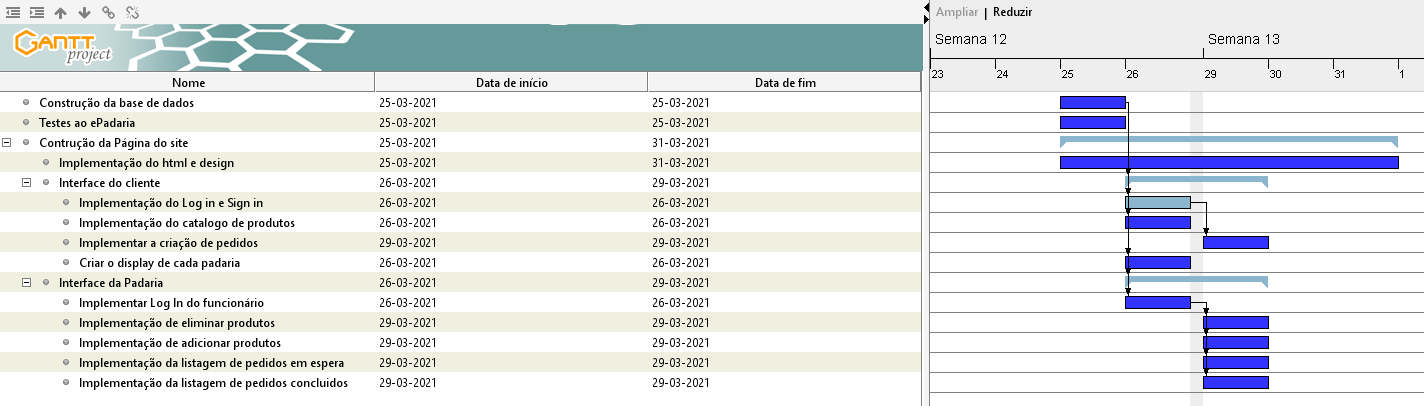
\includegraphics[width=15cm]{gantt}
	\caption{Gantt Poject do ePadaria}
	\label{fig:gantt}
\end{figure}